% Section V: Results. Numbers: results/phase2/tuning/hybrid_mlp.csv (tuning),
% metrics/learning_curves.csv, ablation.csv, cv_seeds.csv (CV), metrics/
% comparison.csv, seeds.csv, error_breakdown.csv, per_phone.csv,
% floor_confusion.csv (test set), tuning/blend.csv and blend.json (the blend);
% Phase 1 rows: results/metrics/. CV = mean over the five user-group folds.
\section{Results}\label{sec:results}

\subsection{Tuning and Training}\label{sec:res-tuning}
Table~\ref{tab:tuning} shows the three position weights. With $\lambda=30$ the
position error is higher (9.51~m, 0.26~m more, about the size of chance between
two runs, Section~\ref{sec:res-ablation}); $\lambda=100$ and $\lambda=300$ are
practically tied (9.2509 and 9.2499~m), and the rule picks $\lambda=300$, which
also finds more floors (81.5\% against 79.9\%).

\begin{table}[t]
  \caption{Tuning the Position Weight $\lambda$ (User-Group CV, Hybrid MLP)}
  \label{tab:tuning}
  \centering
  \footnotesize
  \begin{tabular}{@{}rccc@{}}
    \toprule
    $\lambda$ & Building (\%) & Floor (\%) & Mean 2D error (m) \\
    \midrule
    30 & 99.3 & 82.5 & 9.51 \\
    100 & 99.3 & 79.9 & 9.25 \\
    \textbf{300} & \textbf{99.3} & \textbf{81.5} & \textbf{9.25} \\
    \bottomrule
  \end{tabular}
\end{table}

\begin{figure*}[t]
  \centering
  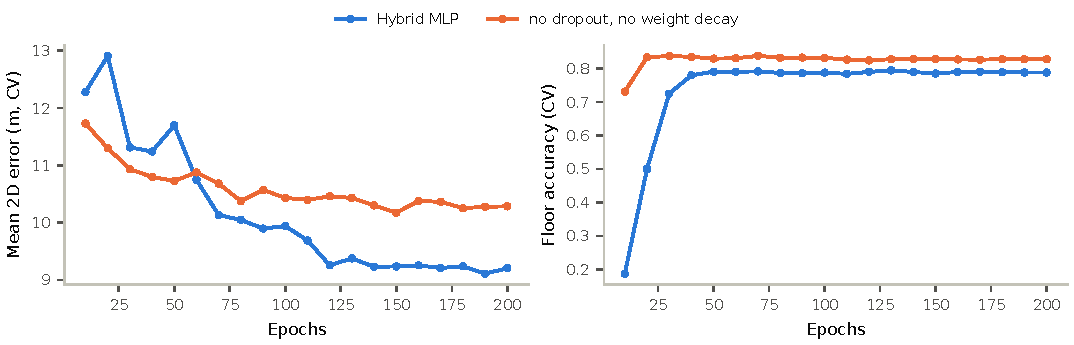
\includegraphics[width=\textwidth]{dl_learning_curves.pdf}
  \caption{CV mean 2D error and floor accuracy during one 200-epoch training
  run, scored every 10 epochs, for the hybrid MLP and for the same network
  without dropout and weight decay. The learning rate falls to 0 along a cosine
  curve, so a point at epoch $k$ is the network part-way through this run, not
  a network trained for $k$ epochs.}
  \label{fig:curves}
\end{figure*}

Fig.~\ref{fig:curves} shows one training run of the ablation study. The
regularized network keeps improving until the learning rate is small and ends
at 9.21~m; without dropout and weight decay it stops improving earlier and ends
at 10.28~m. The regularized network also learns the floors slowly: after 10
epochs it finds only 18.7\% of them (73.1\% without dropout and weight decay, with
the same $\lambda$), and it catches up by epoch 50 (79.0\%).

\subsection{Ablation Study}\label{sec:res-ablation}
Table~\ref{tab:ablation} removes one part of the hybrid MLP at a time (new seed,
same folds). Trained with three seeds, the full network scores
$9.12\pm0.11$~m (8.99 to 9.21~m; the run in the table is the weakest). Every
row is a single run, so the difference between two rows varies by about
$\sqrt{2}\times0.11\approx0.16$~m by chance. Dropout and weight decay matter
most: without them the error rises by 1.08~m, in all five folds. The heard
indicators lower the position error by 0.58~m (worse without them in four
folds), but without them the floor accuracy is higher (84.6\% against 78.8\%):
they help position and cost floors. The effect of hidden WAPs (0.16~m, four
folds) is at the level of chance, and the Phase~1 features do not help (the
error without them is 0.04~m lower). Three single-task networks are better than
the shared network on every task, by 0.30~m and 6.0 floor points (for position,
a single-task network also beat a SIMO-style MLP on this dataset, 8.25 against
9.20~m~\cite{laska2022multitask}), but they need three times as many weights
(1.9 million against 0.65 million) and three trainings.

\begin{table}[t]
  \caption{Ablation Study (User-Group CV): One Change at a Time}
  \label{tab:ablation}
  \centering
  \footnotesize
  \setlength{\tabcolsep}{3pt}
  \begin{tabular}{@{}lcccc@{}}
    \toprule
    Variant & Floor (\%) & 2D (m) & Change (m) & Worse folds \\
    \midrule
    Hybrid MLP (full) & 78.8 & 9.21 & -- & -- \\
    Three single-task nets & 84.8 & 8.90 & $-0.30$ & 0 \\
    No Phase~1 features & 79.5 & 9.17 & $-0.04$ & 2 \\
    No heard indicators & 84.6 & 9.79 & $+0.58$ & 4 \\
    No hidden WAPs & 80.5 & 9.37 & $+0.16$ & 4 \\
    No dropout or weight decay & 82.8 & 10.28 & $+1.08$ & 5 \\
    \bottomrule
  \end{tabular}
\end{table}

\subsection{Phase 1 vs Phase 2 on the Test Set}\label{sec:res-test}
Table~\ref{tab:test} and Fig.~\ref{fig:comparison} compare all models on the
1,111 test scans. The hybrid MLP finds 99.9\% of the buildings (one scan
wrong) and 90.8\% of the floors, with a mean 2D error of 8.32~m. Trained with
five seeds it scores $8.21\pm0.06$~m and $91.7\pm0.7$\% of floors; the reported
run (seed 42) is the weakest of the five on both, so its numbers are slightly
pessimistic, but the seed moves the test error by only about 0.1~m. Its mean
2D error is lower than that of the plain MLP (8.44~m, a gap within the seed
spread; the MLP finds slightly more floors, 90.9\%) and of Phase~1's kNN and
Baseline RF, but not of the Random Forest (7.42~m, 92.2\% of floors) or XGBoost
(7.86~m, 95.2\%). The three single-task networks are the best networks
(8.03~m, 94.1\% of floors). The blend of the Random Forest and the hybrid MLP
reaches 8.10~m and 92.2\% of floors: better than the network, but not than the
forest on position (Section~\ref{sec:res-blend}).

\begin{table*}[t]
  \caption{Test Set Results (1,111 Scans): Phase~1 Models, Phase~2 Networks and the Blend}
  \label{tab:test}
  \centering
  \footnotesize
  \begin{tabular}{@{}llcccccc@{}}
    \toprule
    Phase & Model & Building (\%) & Floor (\%) & MAE $x$ (m) & MAE $y$ (m) & Mean 2D (m) & Median 2D (m) \\
    \midrule
    1 & Baseline RF & 99.8 & 91.2 & 8.68 & 7.40 & 12.52 & 7.70 \\
    1 & kNN & 99.8 & 87.5 & 6.12 & 5.70 & 9.22 & 5.88 \\
    1 & Random Forest & 100.0 & 92.2 & 4.77 & 4.64 & 7.42 & 5.34 \\
    1 & XGBoost & 100.0 & 95.2 & 5.18 & 4.77 & 7.86 & 6.19 \\
    2 & MLP (Wi-Fi inputs only) & 100.0 & 90.9 & 5.72 & 5.11 & 8.44 & 6.33 \\
    2 & Hybrid single-task MLPs & 100.0 & 94.1 & 5.40 & 4.93 & 8.03 & 5.75 \\
    2 & \textbf{Hybrid MLP (final network)} & \textbf{99.9} & \textbf{90.8} & \textbf{5.64} & \textbf{5.06} & \textbf{8.32} & \textbf{6.10} \\
    2 & Blend: Random Forest + hybrid MLP & 100.0 & 92.2 & 5.46 & 4.93 & 8.10 & 5.92 \\
    \bottomrule
  \end{tabular}
\end{table*}

\begin{figure*}[t]
  \centering
  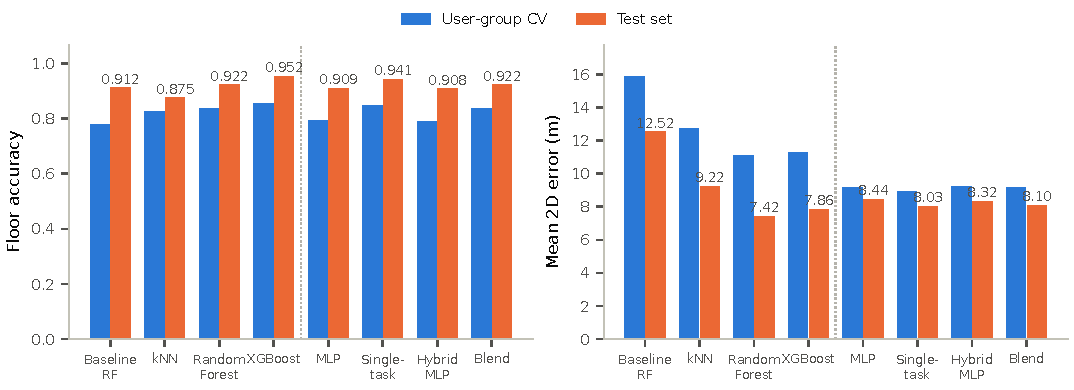
\includegraphics[width=\textwidth]{aml_vs_dl.pdf}
  \caption{Floor accuracy and mean 2D error of every model: user-group CV
  (blue) next to the test set (orange, with values). Phase~1 models are left of
  the dotted line, Phase~2 models right of it.}
  \label{fig:comparison}
\end{figure*}

\emph{CV and the test set disagree.} User-group CV ranked the networks well
ahead of the Random Forest (9.21 against 11.09~m), but on the test set the
order is reversed. All models do better on the test set than in CV, but the
trees gain much more (Random Forest: 11.09 to 7.42~m; hybrid MLP: 9.21 to
8.32~m). Our guess, which we did not test: most test scans lie close to
training positions, where a forest can reuse the training scans almost
directly, while CV holds out whole users, who also walked other places.
Networks are biased towards smooth functions and fit irregular ones less well
than trees~\cite{grinsztajn2022tree}, which may help in new places and cost
accuracy at known ones. With only 16 user groups, a CV ranking is itself
uncertain.

\subsection{The Hybrid Blend}\label{sec:res-blend}
CV chose a forest weight of 0.8 for building, 1.0 for floor (the forest alone)
and 0.1 for position. In CV the blend beats both models on position, with a
mean 2D error of 9.14~m (network alone 9.21~m, forest alone 11.09~m), and finds
as many floors as the forest (83.6\%; network 78.8\%). On the test set it improves the network (8.10 against
8.32~m, 92.2 against 90.8\% of floors, the forest's floors), but not the
forest's position error (7.42~m): because the forest was much worse than the
network in CV, CV gave it only a small weight for position, while on the test
set it is the better of the two. The blend still finds every building, and
88.4\% of its error is on scans with building and floor right.

\subsection{Where the Errors Are}\label{sec:res-errors}
The hierarchical breakdown of the hybrid MLP's test errors: the building is
wrong for one scan (39.80~m error); the building is right but the floor wrong
for 101 scans, 9.1\% (mean 2D error 12.94~m, 14.1\% of the total error); and
85.4\% of the total error is on scans with building and floor right (Random
Forest: 86.2\%). As in
Phase~1, most of the error is the position on the right floor. Of the 102 test
scans with a wrong floor (one of them also in the wrong building), 100 are one
floor off (Fig.~\ref{fig:confusion}), and building~1
is the hardest: 38 of its 143 floor-1 scans are put on floor~2. New phones are
harder for the network too: 9.27~m against 6.62~m on the two phones seen in
training (Random Forest: 8.30 against 5.84~m).

\begin{figure*}[t]
  \centering
  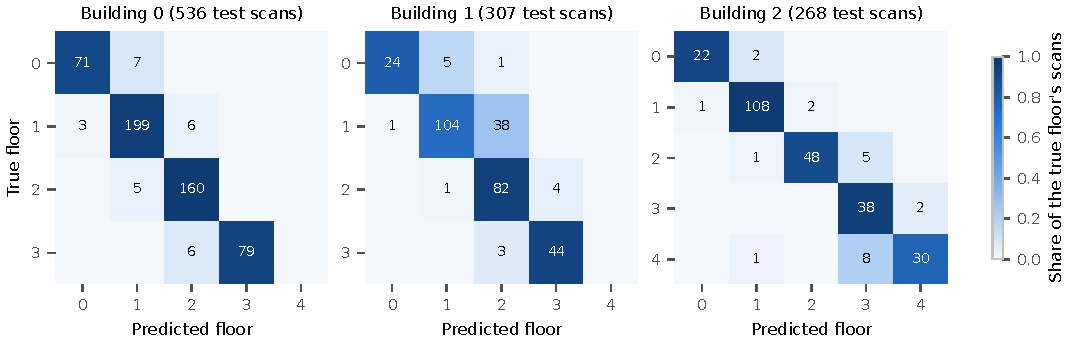
\includegraphics[width=\textwidth]{dl_floor_confusion.pdf}
  \caption{Floor confusion matrices of the hybrid MLP on the test set, one per
  building; colors show the share of each true floor's scans.}
  \label{fig:confusion}
\end{figure*}
